
Process mining \cite{bible} is a field of computer science aiming to reconstruct the latent process model from a manifest event data. Together with the surge of data availability, process mining has become a hot topic in the fields of data science and business intelligence. 

The foundation of all process mining discovery algorithms is the so-called \emph{event log}: A chronologically ordered list of every event recorded in a business system. Event logs have three mandatory feature attributes. \emph{Case ID} represents which case the event belongs to. \emph{Activity} portrays what kind of event happened. \emph{Timestamp} logs the time of occurrence of that specific event. Table \ref{tab:example_event_log} demonstrates a simple example of an event log.

\renewcommand{\arraystretch}{1.25}
\begin{table}[h]
    \centering
	\caption{Example event log.}
    \begin{tabular}{|c|c|c|c|c|}
        \hline
        \textbf{Case ID} & \textbf{Activity} & \textbf{Timestamp} & \textbf{Resource} & \textbf{Cost (Euros)} \\ 
        \hline
        001 & Start process  & 2024-10-01 08:30 & User A & 15 \\ 
        001 & Review data    & 2024-10-01 09:00 & User B & 30 \\ 
        001 & Approve request & 2024-10-01 09:45 & User C & 10 \\ 
        001 & Send email     & 2024-10-01 10:15 & User D & 5  \\ 
        001 & Finish process & 2024-10-01 10:25 & User A & 20 \\
		002 & Start process  & 2024-10-01 11:30 & User A & 15 \\ 
        002 & Review data    & 2024-10-01 11:46 & User B & 30 \\ 
        002 & Finish process & 2024-10-01 12:11 & User A & 10 \\ 
		$\vdots$ & $\vdots$ & $\vdots$ & $\vdots$ & $\vdots$ \\
        \hline
    \end{tabular}
    \label{tab:example_event_log}
\end{table}

The three major branches of process mining are \emph{process discovery}, \emph{conformance checking}, and \emph{process enhancement} \cite{bible}. \emph{Process discovery} is where a process model is extracted from a submitted event log. In \emph{conformance checking}, the quality of the discovered process model is evaluated in terms of various criteria such as fitness, precision, generalization, and simplicity \cite{conformance-checking}. Finally, in the \emph{enhancement} phase, the idea is to extend or improve the existing process model using the data present in the event log.


\section{Motivation}
\label{sec:intro_ssec:motiv}



\begin{comment}
    In this section, you explain to the reader why:

\begin{enumerate}
    \item The problem you are solving is relevant to be solved.
    \item The existing solutions do not solve the problem and/or have significant problems/shortcomings when doing so.
\end{enumerate}
Note that parts of this section are already highlighted in both the abstract and the introduction.
However, in this section, you dive a bit deeper.
In a good motivation, you show a (simple) example on which current methods fail, yet, the method that you are going to describe in this thesis actually yields a better result.

For example, assume that your thesis describes a new \emph{process-discovery} algorithm that is able to handle noise, incomplete behavior, and, on top of that, is able to apply label-splitting.
You can take an (example) event log and show that existing algorithms result in models that are of suboptimal quality.
Finally, you show a model discovered by your fancy algorithm, and, you explain why this model is so much better.
\end{comment}

Business processes are seldom linear. Instead, they are usually a messy, chaotic, intertangled mash of activities where its golden path is meticulously hidden. On top of that, event logs have no guarantee of completeness. The quality of the process model produced by process-discovery techniques is therefore entirely dependent on the quality of its event log.

\subsection{Insights of Enabled Activities}

In an ideal world where perfect process discovery is conceivable, an event log would be \emph{transparent}, containing metadata of structural properties of the corresponding process model, e.g., state information in a Petri net setting. Event logs, however, are usually \emph{opaque} - one cannot identify the underlying process model straight away by solely looking at the log. One must instead utilize process-discovery algorithms to generate corresponding models. By its nature, process event logs primarily focus on what \emph{happened}. However, they often do not take into consideration what \emph{could have happened} instead. An event log is \textit{translucent} if the log contains the information which alternative activities could have potentially taken place instead of the actual activity occurred in the real world. Logs of this nature are called \textit{translucent event logs} and are extremely beneficial to enhance the quality of existing process-discovery algorithms.

Let us consider a small example as motivation. Suppose the underlying model of our business process is represented as the Petri net below.

\begin{figure}[H]
    \centering
    \begin{tikzpicture}
    % Place 1
    \node[place, tokens=1] (p1) at (0,0) {};
    
    % Place 2
    \node[place] (p2) at (3,1) {};

    % Place 3
    \node[place] (p3) at (3,-1) {};

    % Place 4
    \node[place] (p4) at (6,1) {};

	% Place 5
	\node[place] (p5) at (6,-1) {};

    % Place 6
    \node[place] (p6) at (9,0) {};
    
    % Transition a
    \node[transition, minimum width=0.8cm, minimum height=0.8cm, label=center:a] (a) at (1.5,0) {}
        edge[pre]   (p1)
        edge[post]  (p2)
        edge[post]  (p3);
        
    % Transition b
    \node[transition, minimum width=0.8cm, minimum height=0.8cm, label=center:b] (b) at (4.5,1) {}
        edge[pre]   (p2)
        edge[post]  (p4);

    % Transition c
    \node[transition, minimum width=0.8cm, minimum height=0.8cm, label=center:c] (c) at (4.5,-1) {}
        edge[pre]   (p3)
        edge[post]  (p5);
        
    % Transition d
    \node[transition, minimum width=0.8cm, minimum height=0.8cm, label=center:d] (d) at (7.5,0) {}
        edge[pre]   (p4)
		edge[pre]   (p5)
        edge[post]  (p6);
\end{tikzpicture}
\caption{Example business model represented as a Petri net.}
\label{petrinet}

\end{figure}

We play-out the model fifty times and retrieve the event log $\mathcal{L}_1 = [ \langle a, b, c, d \rangle ^{48}, \langle a, c, b, d \rangle^2 ]$ in the process. We can then leverage widely used process-discovery algorithms to rediscover the process model described in Figure \ref{petrinet}. 

This works under the assumption of log completeness, but what would happen if the trace $\langle a, c, b, d \rangle$ occurs so rarely that we weren't able to capture the behavior? Given the log subset $\mathcal{L}_2 = [ \langle a, b, c, d \rangle ^{50}]$, every process-discovery algorithm will return a linear process model. The translucent variant would look like $\mathcal{L}_3 = [ \langle \underline{a}, \underline{b}c,  \underline{c},  \underline{d} \rangle ^{50}]$, where all enabled activities are listed and the executed activity is underscored. Here, the choice situation between activities $b$ and $c$ is clearly visible, thus preventing the linear modelling of our process.

% % In fact, translucent logs make the process-discovery trivial for a certain subclass of process models, for which each state activates a unique set of activities. Such process models are called \textit{lucent process models.} Sound workflow nets that are short-circuited and free-choice belong to this class of process models. Although this seems like a hard restriction, many of the real-life workflow nets modelling business processes are reported to possess the free-choice property \cite{Advances in Quantitative Analysis of Free-Choice Workflow Petri Nets}.

Despite its benefits, lucent models and translucent event logs are relatively new concepts and are therefore scarcely researched. As a result, translucent event logs are hardly available in real-life process logs. This motivates us to devise novel methods to generate translucent event logs from a non-translucent event log.

\subsection{Limitations of Previous Methods}

The problem of embedding translucent information in the event log is relatively new and few methods have been proposed so far. This prompts us to explore new methods to annotate event logs with enabled activities.

Among the previously suggesting methods, one of them involves annotating the event log with activities which are in turn pattern-matched by labeling the user's system interface. This requires manual labor of labeling individual patterns and are rather unrealistic for real-life systems with a sizable variety of system interfaces.

Another method suggests replaying the event log on the provided process model and annotating the enabled activities in the log. This method is more feasible, but the quality of the annotation, i.e., the accuracy of the enabled activities, is heavily dependent on the quality of the process model. As process models returned by process-discovery algorithms, such as the Inductive Miner, tend to be underfitting, the method above will likely take a superset of enabled activities for each event, thereby reducing its accuracy.

% \subsection*{Neglecting the Data-Centered Aspect}
Current methods of translucent log annotation are solely focused on the control-flow aspect, even though the data attributes of event logs also contain valuable information and have an impact on activity enablement.  

\section{Problem Statement}
\label{sec:intro_ssec:probs}

Taking these aforementioned aspects into account, our problem statement can be formulated as the following.

\begin{tcolorbox}[colback=gray!10!white, colframe=black, boxrule=0.5mm, arc=0mm, left=5mm, right=5mm, top=3mm, bottom=3mm]
	\emph{\textbf{Translucent Log Extension:} Given an event log and an auxiliary process model, annotate the event log with translucent information while incorporating the data attributes into the computation.}
\end{tcolorbox}

\section{Research Questions}

In the scope of the thesis, we define the four research questions below: 

\textbf{\emph{RQ1.}} Which techniques can detect enabled activities considering solely the log?

\textbf{\emph{RQ2.}} Which techniques can detect enabled activities considering the log-model pair?

\textbf{\emph{RQ3.}} How do these methods compare to each other in terms of accuracy and runtime?

\textbf{\emph{RQ4.}} How can we design and implement an intuitive, user-friendly tool to demonstrate our results?


\section{Research Goals}

The principal research goal of this thesis paper is to explore different methods to annotate event logs with translucent information. Furthermore, by building a meaningful, easily operable end-user framework dedicated to translucent log annotation, the \textbf{Translucify} framework should be able to evaluate these methods systematically with respect to its accuracy and runtime.

\begin{figure}[H]
    \centering
    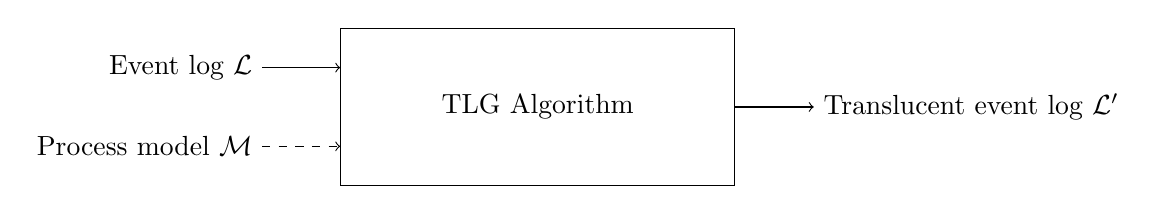
\begin{tikzpicture}

    % Draw the box
    \node[draw, minimum width=5cm, minimum height=2cm, align=center] (box) at (0,0) {TLG Algorithm};

    % Draw the input arrows with labels on the side
    \draw[->] (-3.5,0.5) -- node[pos=0,left] {Event log $\mathcal{L}$} (box.west |- 0.5, 0.5);
    \draw[->, dashed] (-3.5,-0.5) -- node[pos=0, left] {Process model $\mathcal{M}$} (box.west |- -0.5,-0.5);

    % Draw the output arrow with label on the side
    \draw[->] (box.east) -- ++(1,0) node[right] {Translucent event log $\mathcal{L'}$};

	\end{tikzpicture}
    \caption{Workflow of Translucify. The algorithm takes an event log $\mathcal{L}$ and an optional process model $\mathcal{M}$, then returns an annotated translucent event log $\mathcal{L'}$.}
    \label{fig:translucify_workflow}
\end{figure}

We hereby explicitly state that while the generated translucent log could be applied for further use, especially for process discovery to enhance previously discovered models, the exact application of generated translucent event logs is not the scope of this thesis. Instead, our sole focus lies on the log enhancement phase.

\section{Contributions}
\begin{comment}
    In this section, you list the contributions that your thesis makes to our wonderful world (of science).
Again, there is a strong link to the previous section.
Usually, you have achieved your research goals.
Hence, the contributions are concrete statements of the goals you have achieved.
Additionally, your evaluation (most likely also stressed as a goal) is a contribution.
Any implementation or prototype can also be quantified as a contribution.

Some examples:
\begin{itemize}
	\item A systematic literature review covering 35 articles on noise patterns in real event data
	\item A noise detection algorithm based on dynamic programming and symbolic linking
	\item ...
\end{itemize}
\end{comment}


\section{Thesis Structure}

The remainder of this thesis is structured as follows. We first present related work in \cref{chap:related_work}. We then introduce basic mathematical preliminaries in \cref{chap:prelim}. In \cref{chap:method}, the main ideas of translucent event log generation algorithms are presented and thoroughly explained, followed by the implementation specifications in \cref{chap:impl}. The evaluation methods and results are displayed in \cref{chap:eval}. Finally, discussion of the result, further limitations and future perspectives are presented in \cref{chap:discussion}. 